
\chapter{Angular Integration in Excess Functional \label{chpt:fft-spatial}}

As discussed in last chapter, the Fourier transform of the excess
functional gradient is:
\begin{equation}
\hat{\gamma}(\mathbf{k},\mathbf{\Omega}_{1})=\int\mathrm{d}\mathbf{\Omega}_{2}\Delta\hat{\rho}(\mathbf{k},\mathbf{\Omega}_{2})\hat{c}(\mathbf{k},\mathbf{\Omega}_{1},\mathbf{\Omega}_{2})\label{eq:gamma-k}
\end{equation}

It should be pointed out that the direct correlation function (\acs{DCF}),
$\hat{c}(\mathbf{k},\mathbf{\Omega}_{1},\mathbf{\Omega}_{2})$, used
as an input data in eq. (\ref{eq:gamma-k}) is very memory-costly.
In the previous work \citep{gendre_classical_2009,Zhao_2011,borgis_molecular_2012},
the \acs{DCF} bas been stocked in the intermolecular form $\hat{c}(k,\boldsymbol{\omega}_{1},\boldsymbol{\omega}_{2})$
to profit an economy of memory, where $(\boldsymbol{\omega}_{1},\boldsymbol{\omega}_{2})\equiv(\cos\theta_{1},\cos\theta_{2},\phi_{12})$,
and the correspondence of $(\mathbf{\Omega}_{1},\mathbf{\Omega}_{2})$
to $(\boldsymbol{\omega}_{1},\boldsymbol{\omega}_{2})$ is calculated
directly in the code. These works adapt well with linear solvents,
but are proved less powerful for molecular solvent such as water.
However, in the case of full Euler angles intermolecular \acs{DCF}
(fig. \ref{fig:coordinate_systems}), 
\begin{equation}
\hat{c}(k,\boldsymbol{\omega}_{1},\boldsymbol{\omega}_{2})\equiv\hat{c}(k,\cos\theta_{1},\cos\theta_{2},\phi,\psi_{1},\psi_{2})
\end{equation}
neither the storage of $\hat{c}(\mathbf{k},\mathbf{\Omega}_{1},\mathbf{\Omega}_{2})$
which is definitively impossible, nor the direct calculation of correspondence
$(\mathbf{\Omega}_{1},\mathbf{\Omega}_{2})$ to $(\boldsymbol{\omega}_{1},\boldsymbol{\omega}_{2})$
due to the increased complexity that makes it too costly, can be regard
as a possible solution. For instance, with a normal setting of $64^{3}$
spatial grid and a Lebedev quadrature of order 2 (14 angles for $\Theta$
and $\Phi$), and 3 $\Psi$-angles, even if the \acs{DCF} is stocked
in simple precision (complex number), it takes $64^{3}\times42^{2}\times4\,\mathrm{bytes}\times2=3.52\mathrm{GB}$,
and for a Lebedev quadrature of order 5 and correspondingly 5 $\Psi$-angles,
it takes $64^{3}\times250^{2}\times4\,\mathrm{bytes}\times2=131\mathrm{GB}$.
As a normal PC has only 4 to 16 GB of RAM, it can cause a memory leak. 

Therefore, two strategies are developed to treat the full \acs{DCF}
case. The first one is a direct extension of the previous work, which
uses the full intermolecular \acs{DCF} with a more complicate angle
correspondence pre-tabulated in the beginning of the implementation.
The other calculates the \acs{DCF} directly from rotational invariant
projections. Here we give a complete discussion of these two strategies.

\begin{figure}[H]
\begin{centering}
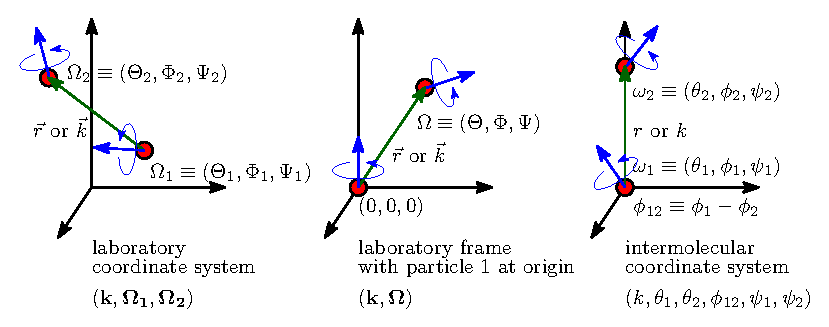
\includegraphics{_figure/coordinate_system}
\par\end{centering}
\caption[Molecules 1 and 2 in different coordinate systems]{Molecules 1 and 2 in different coordinate systems. The laboratory
coordinate system is the system of our grid with a fixed reference
view. When one of the molecules is considered as the reference, e.g.
the solute in the case of $\rho(\mathbf{r},\mathbf{\Omega})$, only
one $\mathbf{\Omega}$ needs to be described. For the intermolecular
frame, in $\mathbf{r}$-space, the $z$ axis is oriented along the
vector $\mathbf{r}_{12}=\mathbf{r}_{2}-\mathbf{r}_{1}$, or in $\mathbf{k}$-space
along the vector $\mathbf{k}$. An orientation $\mathbf{\Omega}\equiv(\Theta,\Phi,\Psi)$
in laboratory frame corresponds to $\boldsymbol{\omega}\equiv(\theta,\phi,\psi)$
in intermolecular frame.\label{fig:coordinate_systems}}
\end{figure}


\section{Using full intermolecular DCF}

For the full \acs{DCF} in intermolecular coordinates system, $\hat{c}(k,\boldsymbol{\omega}_{1},\boldsymbol{\omega}_{2})$,
only 6 variables are needed instead of 9 for $\hat{c}(\mathbf{k},\mathbf{\Omega}_{1},\mathbf{\Omega}_{2})$,
and the storage is considerably reduced. The transform from $\hat{c}(\mathbf{k},\mathbf{\Omega}_{1},\mathbf{\Omega}_{2})$
to $\hat{c}(k,\boldsymbol{\omega}_{1},\boldsymbol{\omega}_{2})$ relies
on the correspondence $\boldsymbol{\omega}(\mathbf{k},\mathbf{\Omega})\equiv(\cos\theta,\phi,\psi)$,
which is here pre-calculated as a table of data.

Finding $\boldsymbol{\omega}$ from $\mathbf{\Omega}$ amounts to
defining the correspondence between the rotation matrices of the two
coordinate systems. The rotation matrix $\mathbf{\hat{R}}_{\mathbf{\Omega}}$
that rotates the solvent molecule from $\mathbf{I}$ to its orientation
$\mathbf{\hat{R}}_{\mathbf{\Omega}}$
\begin{equation}
\mathbf{\hat{R}}_{\mathbf{\Omega}}\mathbf{I}=\mathbf{\hat{R}}_{\mathbf{\Omega}}
\end{equation}
can be expressed by 3 rotation operations $\mathbf{\hat{R}}_{\Phi}$,
$\mathbf{\hat{R}}_{\Theta}$, and $\mathbf{\hat{R}}_{\Psi}$ which
rotate along $z$-$y$-$z$ axes (the same convention as defined in
Messiah \citep{Messiah} and Gray-Gubbins \citep{Gray-Gubbins}):
\begin{align}
\mathbf{\hat{R}}_{\mathbf{\Omega}} & =\left[\begin{array}{ccc}
R_{xx} & R_{xy} & R_{xz}\\
R_{yx} & R_{yy} & R_{yz}\\
R_{zx} & R_{zy} & R_{zz}
\end{array}\right]\\
 & =\left[\begin{array}{ccc}
\cos\Phi & -\sin\Phi & 0\\
\sin\Phi & \cos\Phi & 0\\
0 & 0 & 1
\end{array}\right]\left[\begin{array}{ccc}
\cos\Theta & 0 & \sin\Theta\\
0 & 1 & 0\\
-\sin\Theta & 0 & \cos\Theta
\end{array}\right]\left[\begin{array}{ccc}
\cos\Psi & -\sin\Psi & 0\\
\sin\Psi & \cos\Psi & 0\\
0 & 0 & 1
\end{array}\right]\nonumber \\
 & =\footnotesize\left[\begin{array}{ccc}
\cos\Phi\cos\Theta\cos\Psi-\sin\Phi\sin\Psi & -\cos\Phi\cos\Theta\sin\Psi-\sin\Phi\cos\Psi & \cos\Phi\sin\Theta\\
\sin\Phi\cos\Theta\cos\Psi+\cos\Phi\sin\Psi & -\sin\Phi\cos\Theta\sin\Psi+\cos\Phi\cos\Psi & \sin\Phi\sin\Theta\\
-\sin\Theta\cos\Psi & \sin\Theta\sin\Psi & \cos\Theta
\end{array}\right]\nonumber 
\end{align}
\begin{figure}[b]
\centering{}%
\begin{minipage}[b][1\totalheight][t]{0.55\columnwidth}%
\begin{center}
\includegraphics{_figure/rotation_matrix}\caption{Rotation matrices\label{fig:rotation-matrices}}
\par\end{center}%
\end{minipage}%
\begin{minipage}[b][1\totalheight][t]{0.4\columnwidth}%
\begin{center}
\includegraphics{_figure/rotation_matrix_k}
\par\end{center}
\caption{Rotation to k-frame\label{fig:rotation}}
%
\end{minipage}
\end{figure}

As shown in fig. \ref{fig:rotation-matrices}, the rotation matrix
to transform the \acs{DCF} from the intermolecular coordinates to
laboratory coordinates $\mathbf{\hat{R}}_{\boldsymbol{\omega}}$ can
be written as:
\begin{equation}
\mathbf{\hat{R}}_{\boldsymbol{\omega}}=\mathbf{\hat{R}}_{\mathbf{k}}^{-1}\mathbf{\hat{R}}_{\mathbf{\Omega}}\label{eq:rot-matrix}
\end{equation}
with the rotation matrix related to $\mathbf{k}$ vector:
\begin{equation}
\mathbf{\hat{R}}_{\mathbf{k}}^{-1}=\left[\begin{array}{ccc}
\cos\theta_{k}\cos\phi_{k} & \cos\theta_{k}\sin\phi_{k} & -\sin\theta_{k}\\
-\sin\phi_{k} & \cos\phi_{k} & 0\\
\sin\theta_{k}\cos\phi_{k} & \sin\theta_{k}\sin\phi_{k} & \cos\theta_{k}
\end{array}\right]
\end{equation}

Here we fix $\psi_{k}=0$. $\theta_{k}$ and $\phi_{k}$ are calculated
from Cartesian coordinates ($k_{x}$, $k_{y}$, $k_{z}$). In the
extreme cases where we cannot define $\theta_{k}$ (for $\left\Vert \mathbf{k}\right\Vert =0$)
and $\phi_{k}$ (for $k_{x}^{2}+k_{y}^{2}=0$), we can arbitrarily
fix those angles to zero.

A faster way to find the rotation matrix of $\mathbf{k}$, avoiding
the evaluation of trigonometric functions, is shown in figure \ref{fig:rotation},
where the matrix can be calculated by the cross products of basis
vectors from $z$ axis and $\mathbf{k}$ vector ($\mathbf{k}=\mathbf{e}_{3}^{''}$):
\begin{equation}
\left[\begin{array}{ccc}
\mathbf{e}_{1}^{''} & \mathbf{e}_{2}^{'} & \mathbf{e}_{3}^{''}\end{array}\right]=\left[\begin{array}{ccc}
\mathbf{e}_{1} & \mathbf{e}_{2} & \mathbf{e}_{3}\end{array}\right]\mathbf{\hat{R}_{k}}=\mathbf{\hat{R}_{k}}
\end{equation}

The two ways to calculate $\mathbf{k}$ differ only in the case of
$\hat{\mathbf{k}}=\left[\begin{array}{ccc}
0 & 0 & -1\end{array}\right]^{T}$, where one is the inverse of the other. This is due to the different
definitions of $\phi_{k}$ ($0$ or $\pi$ when $\overrightarrow{k'_{z}}$
superposes with $\overrightarrow{k_{z}}$) in the two cases. Tests
have shown that it has no influence on the final result of the excess
functional evaluation.

The elements of $\mathbf{\hat{R}}_{\boldsymbol{\omega}}$ can be calculated
according to eq. (\ref{eq:rot-matrix}), which possesses the form:
\begin{align}
\mathbf{\hat{R}}_{\boldsymbol{\omega}} & =\left[\begin{array}{ccc}
u_{x} & v_{x} & w_{x}\\
u_{y} & v_{y} & w_{y}\\
u_{z} & v_{z} & w_{z}
\end{array}\right]\\
 & =\footnotesize\left[\begin{array}{ccc}
\cos\phi\cos\theta\cos\psi-\sin\phi\sin\psi & -\cos\phi\cos\theta\sin\psi-\sin\phi\cos\psi & \cos\phi\sin\theta\\
\sin\phi\cos\theta\cos\psi+\cos\phi\sin\psi & -\sin\phi\cos\theta\sin\psi+\cos\phi\cos\psi & \sin\phi\sin\theta\\
-\sin\theta\cos\psi & \sin\theta\sin\psi & \cos\theta
\end{array}\right]\nonumber 
\end{align}

The angles $\boldsymbol{\omega}$ are thus found as:
\begin{eqnarray}
\cos\theta & = & w_{z}\nonumber \\
\phi & = & \arccos(w_{x}/(w_{x}^{2}+w_{y}^{2})^{\frac{1}{2}})\label{eq:omega}\\
\psi & = & \arccos(-u_{z}/(u_{z}^{2}+v_{z}^{2})^{\frac{1}{2}})\nonumber 
\end{eqnarray}

The resulting angles are between normal intervals, $\cos\theta\in\left[-1,1\right]$,
$\phi\in\left[0,2\pi\right]$. As water possesses $\mathrm{C}_{2v}$
symmetry, we take $\psi\in\left[0,\pi\right]$. 

Here the \acs{DCF} $c(k,\boldsymbol{\omega}_{1},\boldsymbol{\omega}_{2})\equiv c(k,\cos\theta_{1},\cos\theta_{2},\phi_{12},\psi_{1},\psi_{2})$
is stored in a discrete set of angles for each value of $k$ (typically
$(8,8,8,8,8)$ in the case of water, which uses the symmetries in
$\mathsection$\ref{subsec:Symmetric-dcf} to reduce the number of
$\phi$ and $\psi$ by two) such that the correspondence from $(\mathbf{\Omega}_{1},\mathbf{\Omega}_{2})$
to $(\boldsymbol{\omega}_{1},\boldsymbol{\omega}_{2})$ usually falls
in between angular grid points of the intermolecular grid. An interpolation
can be done at different orders: zeroth order interpolation, which
directly takes the nearest point, or linear interpolation.

\subsection{Zero-order interpolation of DCF\label{subsec:Zero-order-interpolation-of}}

At this order, for each possible value of $\mathbf{k}$ and $\mathbf{\Omega}$,
the corresponding $\cos\theta$ and $\psi$ which relate to a single
solvent molecule are stored as an index (single precision integer),
which gives the nearest angle in a pre-defined table:
\begin{equation}
\begin{array}{l}
i_{\cos\theta}=\left\lfloor (\cos\theta+1)(n_{\cos\theta}/2)\right\rfloor +1\\
i_{\psi}=\mathrm{mod}(\left\lfloor \psi(n_{\psi}/\pi)\right\rfloor ,n_{\psi})+1
\end{array}
\end{equation}
where $\left\lfloor f\right\rfloor $ is the floor function. For the
angle $\phi$ which relate to two solvent molecules, the operation
$\phi=\phi_{1}-\phi_{2}$ introduces a double error when integer indices
are used, as shown in figure \ref{fig:diff_phi}.

\begin{figure}[h]
\begin{centering}
\includegraphics{_figure/diff_phi}
\par\end{centering}
\caption[$\phi_{1}-\phi_{2}$ distribution]{$\phi_{1}-\phi_{2}$ distribution: Test 0.1 is the direct subtraction
of $\phi$ established in the same way with $\theta$ and $\psi$,
as shown in the top first schema. Test 0.2 tabulates $\phi_{2}$ by
taking the nearest point in another manner, as shown in the second
schema. In test 0.3-0.4, all $\phi$ or only $\phi_{2}$ is doubled.\label{fig:diff_phi}}
\end{figure}

In the actual implementation, as an integer takes 4 bytes and a real
takes 8 bytes, there is no profit to tabulate $\phi$ in integer two
times, thus $\phi$ is stored directly in real.

\subsection{Linear interpolation of DCF\label{subsec:Linear-interpolation-of}}

At this order, $\boldsymbol{\omega}(\mathbf{k},\mathbf{\Omega})$
is stored in double precision. All angles are stored in real number,
and the corresponding \acs{DCF} is calculated as
\begin{equation}
c(\omega)=w_{0}c(\omega_{0})+w_{1}c(\omega_{1})
\end{equation}
where $w_{0}=\dfrac{\omega_{1}-\omega}{\omega_{1}-\omega_{0}}$ and
$w_{1}=\dfrac{\omega-\omega_{0}}{\omega_{1}-\omega_{0}}$. \marginpar{$w$ is the weight, and $\omega$ is the angle set.}Here
$\omega$ is one of the 5 dimensions in $\tilde{\boldsymbol{\omega}}(\mathbf{k},\mathbf{\Omega}_{1},\mathbf{\Omega}_{2})\equiv(\cos\theta_{1},\cos\theta_{2},\phi,\psi_{1},\psi_{2})$,
$\omega_{0}$ and $\omega_{1}$ are the 2 nearest value points, while
other variables are fixed. If we express the weight for each dimension
as $w_{n_{i}}^{i}$ where $i=1,2,3,4,5$ is the $i$th variable, the
total equation with 5 variables is:
\begin{equation}
c(\tilde{\boldsymbol{\omega}})=\left[\sum_{n_{1}=0}^{1}\sum_{n_{2}=0}^{1}\sum_{n_{3}=0}^{1}\sum_{n_{4}=0}^{1}\sum_{n_{5}=0}^{1}\left(\prod_{i}^{5}w_{n_{i}}^{i}c(\tilde{\boldsymbol{\omega}}_{n_{1},n_{2},n_{3},n_{4},n_{5}})\right)\right]\label{eq:interpolation}
\end{equation}

These two equations are available for both interpolation and extrapolation,
where the latter applies, e.g., for $\cos\theta_{1}$ and $\cos\theta_{2}$. 

An error evaluation of the two strategies of interpolation presented
in $\mathsection$\ref{subsec:Zero-order-interpolation-of} and $\mathsection$\ref{subsec:Linear-interpolation-of}
is shown in appendix \ref{chpt:error-evaluation-interpolation-DCF}.
Results demonstrate that the linear interpolation scheme is absolutely
essential. On the other hand, as seen in eq. (\ref{eq:interpolation}),
it is computationally much more expensive than the simple histogram
scheme as it requires $2^{5}=32$ times the number of operations.

\section{Direct calculation of DCF from rotational invariant projections}

Another strategy to calculate $\hat{c}(\mathbf{k},\mathbf{\Omega}_{1},\mathbf{\Omega}_{2})$
is to use the \acs{DCF} expressed in terms of rotational invariant
projections, which takes far less memory than in the intermolecular
function form thanks to their angular independence and symmetric properties. 

\subsection{Using projections in form of $\hat{c}_{\mu\nu}^{mnl}(k)$\label{subsec:Using-projections-in}}

As described by Blum \citep{Blum_I}, $\hat{c}(\mathbf{k},\mathbf{\Omega}_{1},\mathbf{\Omega}_{2})$
can be expanded as
\begin{equation}
\hat{c}(\mathbf{k},\mathbf{\Omega}_{1},\mathbf{\Omega}_{2})=\sum_{mnl\mu\nu}\hat{c}_{\mu\nu}^{mnl}(k)\Phi_{\mu\nu}^{mnl}(\mathbf{\hat{k}},\mathbf{\Omega}_{1},\mathbf{\Omega}_{2})
\end{equation}
where $\Phi_{\mu\nu}^{mnl}(\mathbf{\hat{k}},\mathbf{\Omega}_{1},\mathbf{\Omega}_{2})$
are rotational invariants that depends on both the spatial and angular
coordinates of the two particles (detailed in appendix \ref{chpt:rotational-invariant-expansion}).

For projections of order $n_{\mathrm{max}}=1$ ($n,m\leq1$), the
\acs{DCF} can be expressed in very simple form. Only 4 projections
$\hat{c}^{mnl}(k)$ are independent: $\hat{c}_{\mathrm{S}}\equiv\hat{c}^{000}$,
$\hat{c}_{\mathrm{\Delta}}\equiv\hat{c}^{110}$, $\hat{c}_{\mathrm{D}}\equiv\hat{c}^{112}$
and $\hat{c}^{011}=-\hat{c}^{101}$, with the corresponding rotational
invariants expressed below both in laboratory and intermolecular frames:
\begin{align}
\Phi^{000} & =1\nonumber \\
\Phi^{011} & =i\mathbf{k}\cdot\mathbf{\Omega}_{1}=i\cos\theta_{1}\nonumber \\
\Phi^{101} & =i\mathbf{k}\cdot\mathbf{\Omega}_{2}=i\cos\theta_{2}\nonumber \\
\Phi^{110} & =-\sqrt{3}\mathbf{\Omega}_{1}\cdot\mathbf{\Omega}_{2}=-\sqrt{3}(\sin\theta_{1}\sin\theta_{2}\cos\phi_{12}+\cos\theta_{1}\cos\theta_{2})\nonumber \\
\Phi^{112} & =\sqrt{\frac{3}{10}}\left[3(\mathbf{k}\cdot\mathbf{\Omega}_{1})(\mathbf{k}\cdot\mathbf{\Omega}_{2})-\mathbf{\Omega}_{1}\cdot\mathbf{\Omega}_{2}\right]\\
 & =\sqrt{\frac{3}{10}}\left(2\cos\theta_{1}\cos\theta_{2}-\sin\theta_{1}\sin\theta_{2}\cos\phi_{12}\right)\nonumber 
\end{align}
where the orientations in laboratory frame $\mathbf{\Omega}$ are
here expressed as an orientational vector $\mathbf{\Omega}=(\sin\Theta\cos\Phi,\sin\Theta\sin\Phi,\cos\Theta)$
in the cartesian coordinate system. 

To express the \acs{DCF} at higher orders, the number of \acs{FE}
needed for $\Phi_{\mu\nu}^{mnl}(\mathbf{\hat{k}},\mathbf{\Omega}_{1},\mathbf{\Omega}_{2})$
becomes huge and the \acs{DCF} should be calculated in intermolecular
frame as indicated below.

\subsection{Using projections in form of $\hat{c'}_{\mu\nu,\chi}^{mn}(k)$\label{subsec:Using-projections-in-1}}

Compared to the expression of $\Phi_{\mu\nu}^{mnl}(\mathbf{\hat{k}},\mathbf{\Omega}_{1},\mathbf{\Omega}_{2})$
in laboratory frame (eq. (\ref{eq:definition_rot_invar})), its intermolecular
form has far fewer terms (eq. (\ref{eq:phi_local})), such that
\begin{equation}
\hat{c}(k,\boldsymbol{\omega}_{1},\boldsymbol{\omega}_{2})=\frac{1}{2l+1}\sum_{mn\mu\nu\chi}\hat{c'}_{\mu\nu,\chi}^{mn}(k)r_{\chi\mu}^{m}(\theta_{1})r_{\underline{\chi}\nu}^{n}(\theta_{2})e^{-i\chi(\phi_{12}\equiv\phi_{1}-\phi_{2})}e^{-i\mu\psi_{1}}e^{-i\nu\psi_{2}}\label{eq:dcf-exact}
\end{equation}
where $r$ is the generalized Legendre polynomial, $m,n\leq n{}_{\mathrm{max}}$,
$\left|\mu\right|\leq m$, $\left|\nu\right|\leq n$, and $\chi\in\left[-\mathrm{min}(m,n),\mathrm{min}(m,n)\right]$;
$\underline{\chi}=-\chi$.

$r_{\chi\mu}^{m}(\theta)$, $e^{-i\chi\phi}(\phi)$ and $e^{-i\mu\psi}(\psi)$
can be separately pre-tabulated for each given $\mathbf{k}$, to avoid
repetitive evaluation of each term.

Eq. (\ref{eq:dcf-exact}) replaces the interpolation of eq. (\ref{eq:interpolation})
by an exact formula and it requires the projections $\hat{c}_{\mu\nu,\chi}^{mn}(k)$
to be stored in memory rather than the full angular representation
$\hat{c}(k,\boldsymbol{\omega}_{1},\boldsymbol{\omega}_{2})$. It
also requires the passage from orientations in laboratory frame to
orientations in intermolecular frame, i.e. use of the formulae (\ref{eq:omega})
for each $\mathbf{k}$ vector.
